%% This is the ctufit-thesis example file. It is used to produce theses
%% for submission to Czech Technical University, Faculty of Information Technology.
%%
%% This is version 1.5.8, built 22. 5. 2025.
%% 
%% Get the newest version from
%% https://gitlab.fit.cvut.cz/theses-templates/FITthesis-LaTeX
%%
%%
%% Copyright 2024, Tomas Novacek
%% Copyright 2021, Eliska Sestakova and Ondrej Guth
%%
%% This work may be distributed and/or modified under the
%% conditions of the LaTeX Project Public License, either version 1.3
%% of this license or (at your option) any later version.
%% The latest version of this license is in
%%  https://www.latex-project.org/lppl.txt
%% and version 1.3 or later is part of all distributions of LaTeX
%% version 2005/12/01 or later.
%%
%% This work has the LPPL maintenance status `maintained'.
%%
%% The current maintainer of this work is Tomas Novacek (novacto3@fit.cvut.cz).
%% Alternatively, submit bug reports to the tracker at
%% https://gitlab.fit.cvut.cz/theses-templates/FITthesis-LaTeX/issues
%%
%%

% arara: xelatex
% arara: biber
% arara: xelatex
% arara: xelatex

%%%%%%%%%%%%%%%%%%%%%%%%%%%%%%%%%%%%%%%%%
% CLASS OPTIONS
% language: czech/english/slovak
% thesis type: bachelor/master/dissertation
% electronic (oneside) or printed (twoside), twoside is default
% paragraph - if passed, this optional argument sets paragraphs as the deepest level of headers, styles it, numbers it and adds it to Table of Content. Use with care! Normally, it is considered unwise to use it, since it is too deep.
% colour: bw for black&white OR no option for default colour scheme
%%%%%%%%%%%%%%%%%%%%%%%%%%%%%%%%%%%%%%%%%
\documentclass[czech,bachelor,oneside]{ctufit-thesis}

%%%%%%%%%%%%%%%%%%%%%%%%%%%%%%%%%%
% FILL IN THIS INFORMATION
%%%%%%%%%%%%%%%%%%%%%%%%%%%%%%%%%%
\ctufittitle{Mobilní aplikace pro detekci barev a vizuální návrh barevných schémat} % replace with the title of your thesis
\ctufitauthorfull{Šárka Prokopová} % replace with your full name (first name(s) and then family name(s) / surname(s)) including academic degrees
\ctufitauthorsurnames{Prokopová} % replace with your surname(s) / family name(s)
\ctufitauthorgivennames{Šárka} % replace with your first name(s) / given name(s)
\ctufitsupervisor{doc.\,Ing.\,Marek Suchánek,\,Ph.D. et Ph.D.} % replace with name of your supervisor/advisor (include academic degrees)
\ctufitdepartment{Katedra softwarového inženýrství} % replace with the department of your defence
\ctufitprogram{Informatika} % replace with your study program
\ctufitspecialisation{Softwarové inženýrství} % replace with your specialisation
\ctufityear{2025} % replace with the year of your defence
\ctufitdeclarationplace{Praze} % replace with the place where you sign the declaration
\ctufitdeclarationdate{\today} % replace with the date of signature of the declaration
\ctufitabstractCZE{Tato bakalářská práce se věnuje vývoji multiplatformní mobilní aplikace pro detekci barev a vizuální návrh barevných schémat s dodržením tradičních postupů softwarového inženýrství. Součástí práce je analýza teorie barev, vnímání barev spolu s představením známých barevných sad a popsáním tvorby barevných palet. Provedena je také rešerše existujících řešení a využití metod rozšířené reality.

Na základě analýzy jsou sestaveny požadavky aplikace, dle nichž se zrealizoval návrh. Ten je doprovázen implementací aplikace a jejím testováním. Konec práce se věnuje zhodnocení výsledků a popisu možného rozvoje aplikace.

Výstupem této práce je funkční mobilní aplikace umožňující rozpoznávat barvy a na jejich základě vytvářet barevné palety.}
\ctufitabstractENG{This bachelor thesis focuses on the development of a multiplatform mobile application for colour detection and visual design of colour schemes following traditional software engineering principles. The thesis includes an analysis of colour theory, colour perception 
along with an introduction of recognized colour sets and a description of the creation of
colour palettes. A survey of existing solutions and the use of augmented reality methods is also presented.

On the basis of the analysis, the application requirements are established, according to which the design is developed. This is followed by the implementation of the application and its testing.
The end of the thesis is dedicated to the evaluation of the results and description of the possible development of the application.

The output of this work is a functional mobile application that enables the recognition of
colours and to create colour palettes based on the colours.}
\ctufitkeywordsCZE{teorie barev, vnímání barev, mobilní aplikace, AR, extrakce barev, barevné palety}
\ctufitkeywordsENG{colour theory, perception of colours, mobile application, AR, colour extraction, colour palettes}
%%%%%%%%%%%%%%%%%%%%%%%%%%%%%%%%%%
% END FILL IN
%%%%%%%%%%%%%%%%%%%%%%%%%%%%%%%%%%

%%%%%%%%%%%%%%%%%%%%%%%%%%%%%%%%%%
% CUSTOMIZATION of this template
% Skip this part or alter it if you know what you are doing.
%%%%%%%%%%%%%%%%%%%%%%%%%%%%%%%%%%

\RequirePackage{iftex}[2020/03/06]
\iftutex % XeLaTeX and LuaLaTeX
    \RequirePackage{ellipsis}[2020/05/22] %ellipsis workaround for XeLaTeX
\else
    \errmessage{Only compilation with XeLaTeX or LuaLaTeX is allowed}
    \stop
\fi

% hyperlinks
\hypersetup{
    pdfpagelayout=TwoPageRight,
    colorlinks=false,
    allcolors=decoration,
    pdfborder={0 0 0.1}
}

% uncomment the following to hide all hyperlinks
%\hypersetup{hidelinks}

% uncomment the following to change the colour of all hyperlinks to CTU blue
%\hypersetup{allbordercolors=decoration}

\RequirePackage{pdfpages}[2020/01/28]

%%%%%%%%%%%%%%%%%%%%%%%%%%%%%%%%%%
% CUSTOMIZATION of this template END
%%%%%%%%%%%%%%%%%%%%%%%%%%%%%%%%%%


%%%%%%%%%%%%%%%%%%%%%%
% PACKAGES SETTINGS
% You may choose to modify this part.
%%%%%%%%%%%%%%%%%%%%%%
\usepackage{dirtree}
\usepackage{lipsum,tikz}
\usepackage[style=iso-numeric]{biblatex}
\addbibresource{text/bib-database.bib}
\usepackage{xurl}
\usepackage{listings} % typesetting of sources
%\usepackage{minted}
\usepackage{csquotes}

%%%%%%%%%%%%%%%%%%%%%%
% PACKAGES SETTINGS END
%%%%%%%%%%%%%%%%%%%%%%

\begin{document}
\frontmatter\frontmatterinit % do not remove these two commands

\thispagestyle{empty}\maketitle\thispagestyle{empty}\cleardoublepage % do not remove these four commands

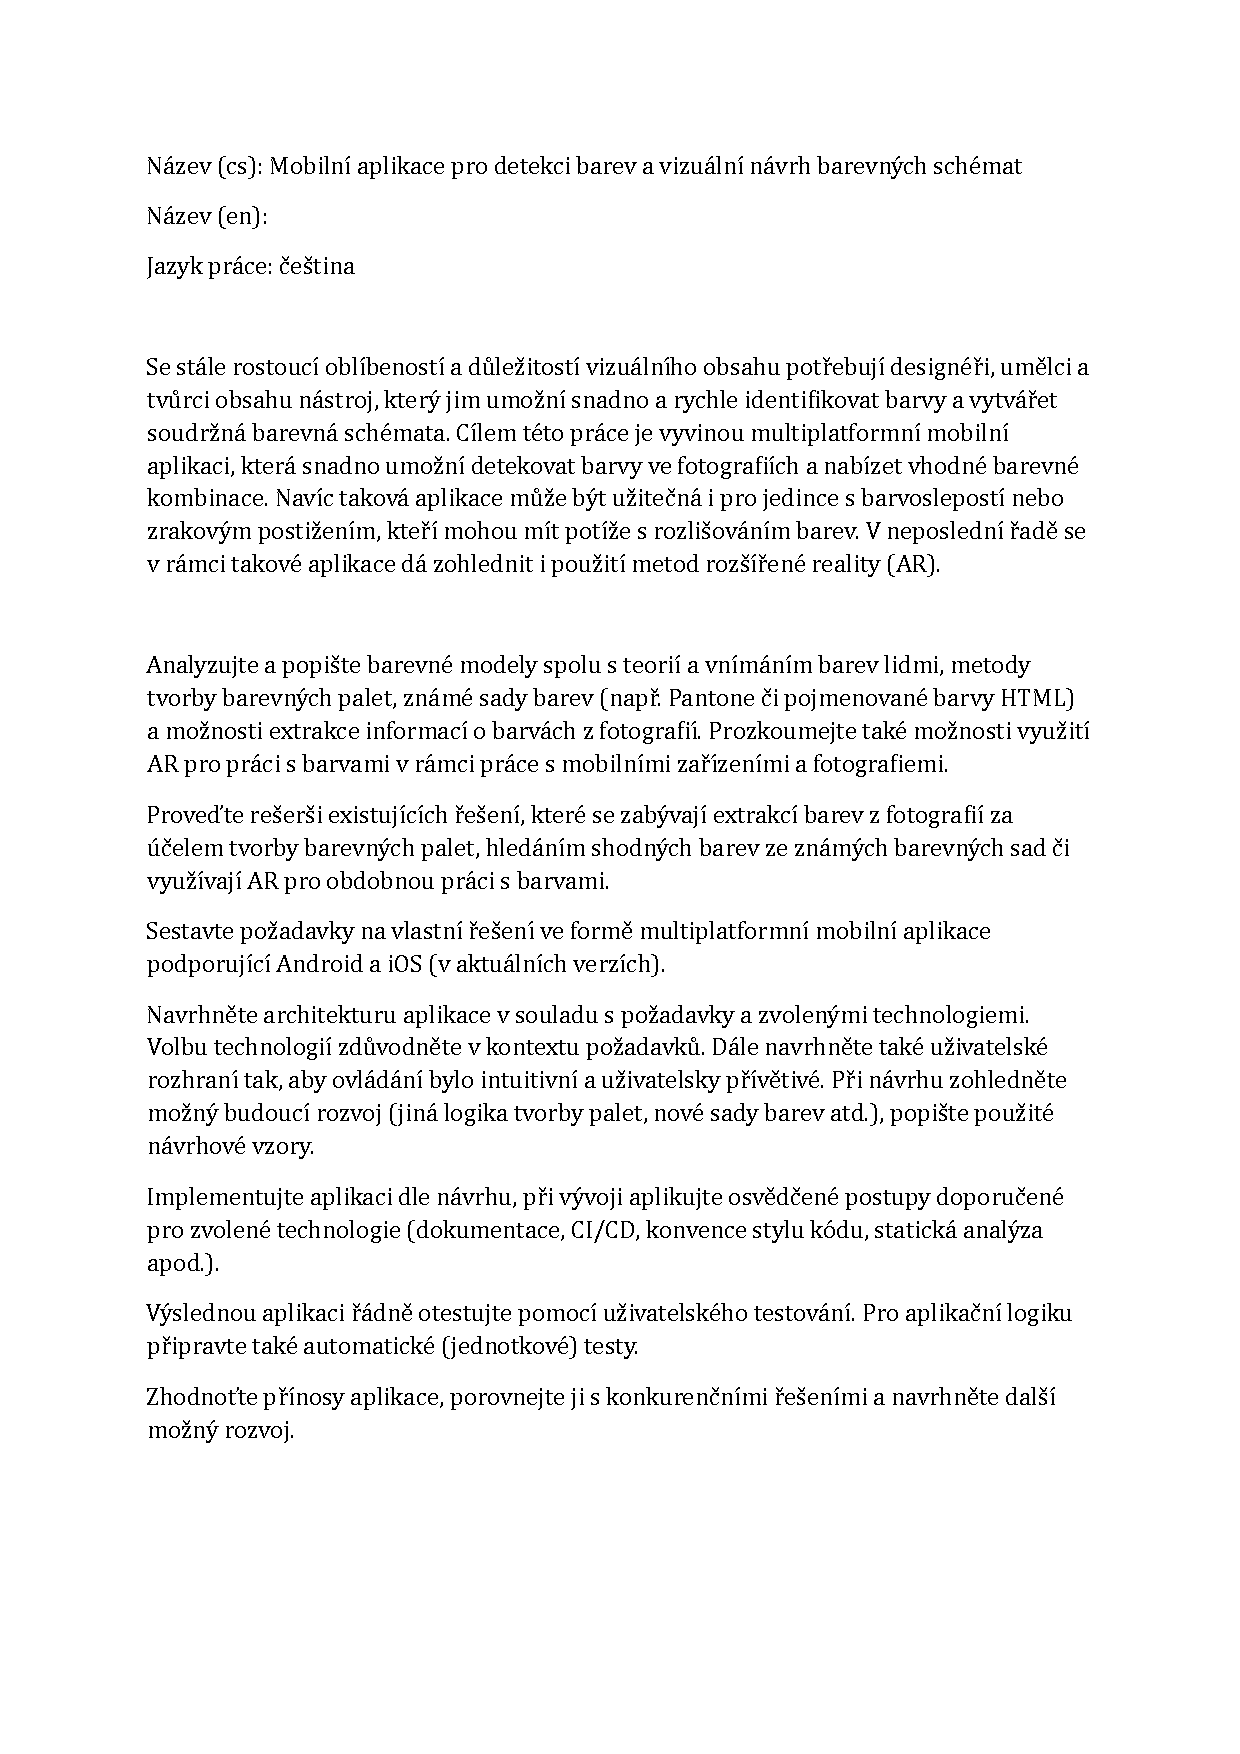
\includepdf[pages={1-}]{assignment.pdf} % replace this file with your thesis assignment generated from ProjectsFIT
% TODO change font

\imprintpage % do not remove this command
\stopTOCentries
%%%%%%%%%%%%%%%%%%%%%%
% list of other contents END
%%%%%%%%%%%%%%%%%%%%%%

%%%%%%%%%%%%%%%%%%%
% ACKNOWLEDGMENT
% FILL IN / MODIFY
% This is a place to thank people for helping you. It is common to thank your supervisor.
%%%%%%%%%%%%%%%%%%%
\begin{acknowledgmentpage}
	Chtěl bych poděkovat především 
\end{acknowledgmentpage}
%%%%%%%%%%%%%%%%%%%
% ACKNOWLEDGMENT END
%%%%%%%%%%%%%%%%%%%


%%%%%%%%%%%%%%%%%%%
% DECLARATION
% FILL IN / MODIFY
%%%%%%%%%%%%%%%%%%%
% INSTRUCTIONS
% ENG: choose one of approved texts of the declaration. DO NOT CREATE YOUR OWN. Find the approved texts at https://courses.fit.cvut.cz/SFE/download/index.html#_documents (document Declaration for FT in English)
% CZE/SLO: Vyberte jedno z fakultou schvalenych prohlaseni. NEVKLADEJTE VLASTNI TEXT. Schvalena prohlaseni najdete zde: https://courses.fit.cvut.cz/SZZ/dokumenty/index.html#_dokumenty (prohlášení do ZP)
\begin{declarationpage}
	Prohlašuji, že jsem předloženou práci vypracovala samostatně a že jsem uvedla veškeré použité
informační zdroje v souladu s Metodickým pokynem o dodržování etických principů při přípravě
vysokoškolských závěrečných prací.

Beru na vědomí, že se na moji práci vztahují práva a povinnosti vyplývající ze zákona č. 121/2000 Sb.,
autorského zákona, ve znění pozdějších předpisů, zejména skutečnost, že České vysoké učení
technické v Praze má právo na uzavření licenční smlouvy o užití této práce jako školního díla podle §
60 odst. 1 citovaného zákona.
\end{declarationpage}
%%%%%%%%%%%%%%%%%%%
% DECLARATION END
%%%%%%%%%%%%%%%%%%%

% Use one of the two following commands. The first prints abstracts+keywords on two pages, the second puts them on one page (if possible). \printonepageabstract can also accept optional argument that specifies a vertical space before both abstracts (the default is 18 mm).
\printtwopageabstract
%\printonepageabstract 

%%%%%%%%%%%%%%%%%%%
% SUMMARY
% FILL IN / MODIFY
% OR REMOVE ENTIRELY (upon agreement with your supervisor)
% (appropriate to remove in most theses)
%%%%%%%%%%%%%%%%%%%
% \begin{summarypage}
% \section*{Summary section}
% 
% \lipsum[1][1-8]
% 
% \section*{Summary section}
% 
% \lipsum[2][1-6]
% 
% \section*{Summary section}
% 
% \lipsum[3]
% 
% \section*{Summary section}
% 
% \lipsum[2]
% 
% \section*{Summary section}
% 
% \lipsum[1][1-8] Lorem lorem lorem.
% \end{summarypage}
%%%%%%%%%%%%%%%%%%%
% SUMMARY END
%%%%%%%%%%%%%%%%%%%

\tableofcontents % do not remove this command
%%%%%%%%%%%%%%%%%%%%%%
% list of other contents: figures, tables, code listings, algorithms, etc.
% add/remove commands accordingly
%%%%%%%%%%%%%%%%%%%%%%
\listoffigures % list of figures
\begingroup
\let\clearpage\relax
\listoftables % list of tables. Remove if you do not have any.
\thectufitlistingscommand{} % list of code listings. Remove if you do not have any.
\thectufitlistofalgorithmscommand{} % list of algorithm pseudocodes defined using the algorithm package.
\endgroup

%%%%%%%%%%%%%%%%%%%
% ABBREVIATIONS
% FILL IN / MODIFY
% OR REMOVE ENTIRELY
% List the abbreviations in lexicography order.
%%%%%%%%%%%%%%%%%%%
\chapter{\thectufitabbreviationlabel}

\begin{tabular}{rl}
	AR   & Augmented Reality                 \\
	FA    & Finite Automaton
\end{tabular}
%%%%%%%%%%%%%%%%%%%
% ABBREVIATIONS END
%%%%%%%%%%%%%%%%%%%
\resumeTOCentries
\mainmatter\mainmatterinit % do not remove these two commands
%%%%%%%%%%%%%%%%%%%
% THE THESIS
% MODIFY ANYTHING BELOW THIS LINE
%%%%%%%%%%%%%%%%%%%

% Do not forget to include Introduction
%---------------------------------------------------------------
\chapter*{Úvod}\addcontentsline{toc}{chapter}{Úvod}\markboth{Úvod}{Úvod}
Barvy a vnímání barev je i přes její důkladné zkoumání v historii stále velmi subjektivní záležitostí. 
Přesto se v průběhu času některým teoretikům, vědcům a filozofům podařilo stanovit určitá pravidla a vlastnosti barev,
které se ve společnosti hojně využívají. Ať už se jedná o předpokládaný umělecký průmysl, v tomto smyslu 
nejen malba či kresba, využití v psychologii, digitálním odvětví, marketingu, či dokonce politice, barvy jsou 
důležitým aspektem, díky kterému můžeme v lidech probouzet emoce, prohlubovat naše myšlenky, v určitých případech 
je využívat také jako nástroj manipulace.

Barvy působí v nervovém systému. Ne každý však má možnost barvy vidět. Je tedy otázkou, jak se takový člověk může 
přizpůsobit dnešní společnosti a zda je možné od společnosti takovému člověku porozumět.

Hlavním cílem této bakalářské práce je proto vyvinout multiplatformní aplikaci, která s pomocí rozšířené reality umožní
rozeznávat barvy objektů v reálném světě a vytvářet další barevné palety. Díky této aplikaci mohou lidé s poruchou vnímání barev
rozlišovat barvy a lépe chápat návaznost na další odstíny. Zároveň je aplikace pomocníkem, díky kterému mohou umělci, tvůrci obsahu
a designéři rychle detekovat barvy a vytvářet soudržná schémata.

Již existující řešení se soustředí většinou pouze na jediný aspekt, buď pouhé rozeznávání barev na fotografii či tvorbu palet na základě stanovené barvy.
Pro uživatele právě sjednocení těchto funkcionalit umožňuje správné porozumění barvám a jejich vnímání. Práce se zabývá analýzou, návrhem a implementací 
aplikace podle tradičních postupů softwarového inženýrství.

TODO kapitoly
\chapter{Cíl práce}
Hlavním cílém této práce je vývoj multiplatformní aplikace pro detekci barev a tvorbu barevných schémat
za použití programovacího jazyka TODO, a to dle tradičních postupů softwarového inženýrství. Práce se tedy soustředí
na analýzu, sestavení požadavků, návrh, implementaci a následné testování.

Prvním bodem je analýza teorie barev, vnímání barev a popsání známých barevných sad a tvorby palet.
Současně se analýza zabývá extrakcí informací z fotografií, a nakonec také využitím AR pro práci s 
mobilním zařízením a fotografiemi.

V další části se budeme věnovat rozborem existujících řešení, které detekují barvy z fotografií či tvoří barevná schémata 
na základě stanovených barev.

Dále sestavíme požadavky a případy užití naší výsledné aplikace. Navážeme návrhem aplikace, tvorbou architektury a přípravou konceptu
uživatelského rozhraní. Dle tohoto návrhu proběhne implementace aplikace a následné testování.

Nakonec vyhodnotíme výslednou aplikaci spolu s dílčími cíli této práce, prodiskutujeme přínos a případný možný rozvoj aplikace.
\setcounter{page}{1}
% uncomment the following line to create an unnumbered chapter
%\chapter*{Introduction}\addcontentsline{toc}{chapter}{Introduction}\markboth{Introduction}{Introduction}
%---------------------------------------------------------------


\chapter{Analýza}
\begin{chapterabstract}
První kapitola je věnována analýze, jenž je potřebná pro získání potřebných informací
a popsání požadavků softwarového produktu. Díky analýze se můžeme v následující kapitole
věnovat návrhu.

Následující stránky jsou věnovány analýze teorie barev a vnímání barev lidmi. Následně
je věnována pozornost známým barevným sadám a tvorbě barevných palet, extrakcí informací z fotografie
a využití AR k této extrakci. 

Prostor je věnován také existujícím aplikacím s podobnými funkcionalitami, díky kterým si upřesníme a definujeme
funkční a nefunkční požadavky. Na závěr specifikujeme požadavky pomocí modelu případů užití.
\end{chapterabstract}

\section{Teorie barev}
Teorie barev by se dala popsat jako soubor postupů a pravidel zahrnující 
používání primárních pigmentových barev, vytváření barevné harmonie, míchání barev
a jejich aplikaci.

Abychom se však mohli věnovat samotným teoriím a určit postupy, se kterými budeme k této práci
přistupovat, je třeba začít s úplnmými základy a definovat si, co vlastně je barva a jak je vnímána
lidským okem.


\subsection{Barva}
Vnímání barev je velmi subjektivní a již od dob Aristotela nám jejich zkoumání nepřineslo
jednotný názor, který by přesně definoval barvu.
Ten založil své poznatky na pozorování slunečního světla, které při odrazu či průchodu objektem
snižuje svou intenzitu nebo je ztmaveno. Vnímal tak barvu jako mísení, míchání, superpozici či juxtapozici
černé a bílé \cite{goethe1840}.

Tento názor se však brzy setkal s kritikou a byl nahrazen novými poznatky od dalších teoretiků.
% Newton, Young, Fresnel, Goethe - zkoumání barev (goethe1840)
% https://books.google.cz/books?hl=en&lr=&id=mujNEAAAQBAJ&oi=fnd&pg=PP13&dq=colour+definition&ots=ECMtqQBf1F&sig=-kCLAYmN6owutngTKMQAJ4Fu2fc&redir_esc=y#v=onepage&q&f=false
% https://d1wqtxts1xzle7.cloudfront.net/112207887/jaic_v32_01-libre.pdf?1709866938=&response-content-disposition=inline%3B+filename%3DColour_theory_Definition_fields_and_inte.pdf&Expires=1752252945&Signature=ZfOn9uc-IsbJP3TrC5MvZV4lSsAOte25rIBlngEMk7LidfCjxXVDtY9tmgN8RPonzWEm4AD0TRa-vkG0SGxMuVksHhNWawTge-7yJNuDxPnS5vOLtoCdWxS3Qpb1Uj1qdG~UnhJq8XXZFIubw9iDNmgUWR0fhSkD~ejasDRYdj-~ZjkHxcYEVLaazY~OFY3QhmTVcZ25B1bzPfnxpwZjDOMPBVPJX397~6qY~0ZsyctLy0jzs8ehTZahxoXmJz8vCDESfASXwe~4IDfXkmWs-2u1JjHVFVDsWb-HVVp~witzDU-VBO0odEnlIta0~WRoEeWiA6oyjz893LdCmRO8iw__&Key-Pair-Id=APKAJLOHF5GGSLRBV4ZA
% další research pro historii a vývoj názorů, odkud a co je barva 
% https://www.pantone.com/articles/color-fundamentals/what-is-color#:~:text=Color%20is%20defined%20as%20the,others%20are%20absorbed%20by%20it.
% pantone stránka - moderní definice barvy, dnešní chápání 

\subsubsection{Vlastnosti barev}

\subsection{Oko a barevné vidění}
% https://is.muni.cz/th/gpxge/Diplomova_prace.pdf
% struktura oka, tyčinky - černobílé, čípky - barevné vidění, proces předávání informace do mozku
% https://www.mendeley.com/catalogue/a9dda4be-621f-3d6f-b83d-343556b66070/
% trichromatické vidění - long(reddish), medium (greenish), and short (bluish) vawelenghts
% rozpoznávání barev v průběhu života
% https://dspace.cvut.cz/bitstream/handle/10467/91222/FBMI-BP-2020-Soukup-Jan-prace.pdf?sequence=-1&isAllowed=y
% teorie vnímání barev,  Young-Helmholtzova - tři typy čípků, Heringova teorie - proces
% spojení obou teorií - Dvoustupňová

\subsection{Teorie barev}

\subsection{Poruchy barevného vidění}
\section{Barevné sady a tvorba barevných palet}
\section{Extrakce informace z fotografie a AR}
\section{Rešerše existujících řešení}
\section{Požadavky}
\section{Model případu užití}

\subsection{Diagram případů užití}
% Modelové situace vizualizující funkční požadavky
% uživatel - Použití nápovědy, identifikace barvy, uložení fotografie, uložení a odstranění barvy, vyhledání barvy,
% umístění objektu do AR, získání barevných schémat

\subsection{Popis případů užití}


\section{Doménový model}

%%%%%%%%%%%%%%%%%%%%%%%%%%%%%%%%%
% alternative using package minted for source highlighting
% package minted requires execution with `-shell-escape'
% e.g., `xelatex -shell-escape ctufit-thesis.tex'
% \begin{listing}
% \begin{minted}{C}
%     #include<stdio.h>
%     #include<iostream>
%     // A comment
%     int main(void)
%     {
%         printf("Hello World\n");
%         return 0;
%     }
% \end{minted}
% \caption{Zbytečný kód}\label{list:8-6}
% \end{listing}
% %%%%%%%%%%%%%%%%%%%%%%%%%%%%%%%%%

\chapter{Návrh}
\begin{chapterabstract}
Návrh aplikace
\end{chapterabstract}

\section{Technologie}
% react native, Viro AR, Expo
\section{Architektura}
% component-based architektura
\section{Uživatelské rozhraní}



\chapter{Implementace}
\input{text/chapters/3_implementation/implementation.tex}

\chapter{Testování}
\input{text/chapters/4_testing/testing.tex}

\chapter{Vyhodnocení a další rozvoj}
\input{text/chapters/5_evaluation/evaluation.tex}

\chapter*{Závěr}\addcontentsline{toc}{chapter}{Závěr}\markboth{Závěr}{Závěr}
\chapter*{Literatura}\addcontentsline{toc}{chapter}{Literatura}\markboth{Literatura}{Literatura}
 % include `text.tex' from `text/' subdirectory

\appendix\appendixinit % do not remove these two commands

\chapter{Ukázky}


Sem přijde to, co nepatří do hlavní části. - přílohy TODO
 % include `appendix.tex' from `text/' subdirectory

\backmatter % do not remove this command

\printbibliography % print out the BibLaTeX-generated bibliography list

\chapter{Obsah příloh}
% Contents of the attachment

	\dirtree{%
		.1 /.
		.2 readme.txt\DTcomment{stručný popis obsahu média}.
		.2 exe\DTcomment{adresář se spustitelnou formou implementace}.
		.2 src.
		.3 impl\DTcomment{zdrojové kódy implementace}.
		.3 thesis\DTcomment{zdrojová forma práce ve formátu \LaTeX{}}.
		.2 text\DTcomment{text práce}.
		.3 thesis.pdf\DTcomment{text práce ve formátu PDF}.
	}
 % include `medium.tex' from `text/' subdirectory

\end{document}
